\section{Giải pháp}

\subsection{A/B Test là gì}

\begin{frame}
	\begin{columns}
		% Column 1
		\begin{column}{0.5\textwidth}
			\begin{block}{A/B Test là gì}
				\alert{A/B Testing} (hay còn được gọi là split testing hay bucket testing) là một phương pháp để so sánh giữa các biến thể của một thuật toán hoặc ứng dụng nào đó, từ đó tìm ra được biến thể nào có hiệu quả tốt hơn.
			\end{block}
			\begin{block}{Ứng dụng của \alert{A/B Testing}}
				\begin{itemize}
					\item Xây dựng Website
					\item Email Marketing
					\item Quảng Cáo và Bán Hàng
					\item Thiết kế Ứng dụng di động
				\end{itemize}
			\end{block}
		\end{column}
		% Column 2
		\begin{column}{0.5\textwidth}
			\begin{block}{Cách hoạt động của A/B Test}
				\alert{A/B Testing} về cơ bản là một cuộc thử nghiệm mà trong đó, hai hoặc nhiều biến thể của trang được hiển thị cho người dùng một cách ngẫu nhiên. Và kết quả của hành động đó sẽ được thể hiên qua conversion rate (tỉ lệ chuyển đổi), từ đó phân tích thống kê được sử dụng để xác định biến thể nào hoạt động tốt hơn cho mục tiêu chuyển đổi nhất định.
			\end{block}
		\end{column}
	\end{columns}
\end{frame}

% \subsection{Cách hoạt động của A/B Test}

% \begin{frame}{Cách hoạt động của A/B Test}
% 	\alert{A/B Testing} về cơ bản là một cuộc thử nghiệm mà trong đó, hai hoặc nhiều biến thể của trang được hiển thị cho người dùng một cách ngẫu nhiên. Và kết quả của hành động đó sẽ được thể hiên qua conversion rate (tỉ lệ chuyển đổi), từ đó phân tích thống kê được sử dụng để xác định biến thể nào hoạt động tốt hơn cho mục tiêu chuyển đổi nhất định.
% \end{frame}

% \subsection{Ứng dụng của A/B Test}

% \begin{frame}{Ứng dụng của A/B Test}
% 	\alert{A/B Testing} có các ứng dụng sau đây
% 	\begin{itemize}
% 		\item Xây dựng Website
% 		\item Email Marketing
% 		\item Quảng Cáo và Bán Hàng
% 		\item Thiết kế Ứng dụng di động
% 	\end{itemize}
% \end{frame}

\subsection{Cấu trúc A/B Test}

\begin{frame}{Cấu trúc A/B Test}
	\begin{description}
		\item[Product] Phân tách nghiệp vụ lớn
		\item[Layer] Phân tách nghiệp vụ nhỏ
		\item[Experiment] Đại diện cho một thí nghiệm
		\item[Test Group] Đại diện cho một biến thể của một thí nghiệm
		\item[Parameter] Đại diện cho các đặc tính của một biến thể
	\end{description}
	\begin{figure}
		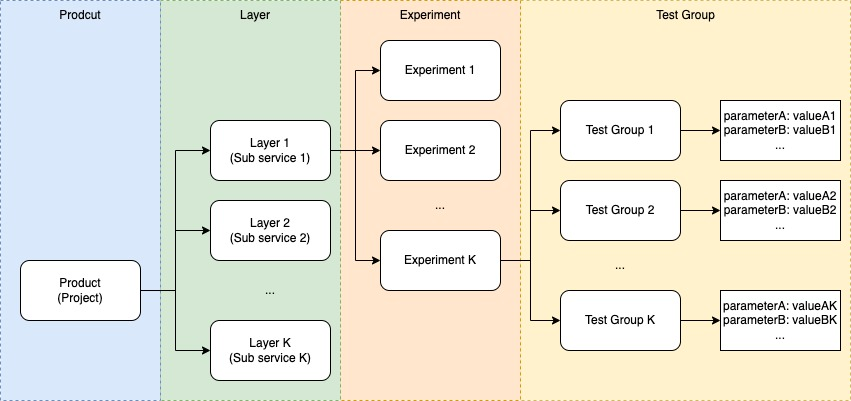
\includegraphics[height = 0.3\textwidth,width = 1\textwidth]{overview-ab-testing}
	\end{figure}
\end{frame}

\begin{frame}
	\begin{columns}
		% Column 1
		\begin{column}{0.5\textwidth}
			\begin{block}{Product}
				\begin{itemize}
					\item Product dùng để phân tách giữa nghiệp vụ lớn
					\item Chỉ có thể sử dụng một Product cho một đối tượng
				\end{itemize}
			\end{block}
			\begin{block}{Ví dụ Product}
				MobileApp, Advertisement, Website, etc..
			\end{block}
			\begin{block}{Ví dụ Layer}
				Giao diện, Recall, Rerank, etc..
			\end{block}
		\end{column}
		% Column 2
		\begin{column}{0.5\textwidth}
			\begin{block}{Layer}
				\begin{itemize}
					\item Layer dùng để phân tách các nghiệp vụ nhỏ trong một Product
					\item Có thể sử dụng nhiều Layer đồng thời cho một đối tượng
					\item Sở hữu 100\% lượng truy cập
					\item Có 2 loại hash strategy để quyết định Experiment
					      \begin{itemize}
						      \item Dùng UserId
						      \item Dùng SessionId
					      \end{itemize}
				\end{itemize}
			\end{block}
		\end{column}
	\end{columns}
\end{frame}

% \begin{frame}{Product}
% 	\begin{block}{Định nghĩa}
% 		\begin{itemize}
% 			\item Product dùng để phân tách giữa nghiệp vụ lớn
% 			\item Chỉ có thể sử dụng một Product cho một đối tượng
% 		\end{itemize}
% 	\end{block}
% 	\begin{block}{Ví dụ}
% 		MobileApp, Advertisement, Website, etc..
% 	\end{block}
% 	\begin{figure}
% 		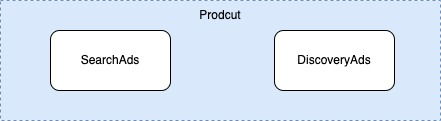
\includegraphics[height = 0.2\textwidth,width = 0.8\textwidth]{product}
% 	\end{figure}
% \end{frame}

% \begin{frame}{Layer}
% 	\begin{block}{Định nghĩa}
% 		\begin{itemize}
% 			\item Layer dùng để phân tách các nghiệp vụ nhỏ trong một Product
% 			\item Có thể sử dụng nhiều Layer đồng thời cho một đối tượng
% 			\item Sở hữu 100\% lượng truy cập
% 			\item Có 2 loại hash strategy để quyết định Experiment
% 			      \begin{itemize}
% 				      \item Dùng UserId
% 				      \item Dùng SessionId
% 			      \end{itemize}
% 		\end{itemize}
% 	\end{block}
% 	\begin{block}{Ví dụ}
% 		Giao diện, Recall, Rerank, etc..
% 	\end{block}
% \end{frame}

\begin{frame}
	\begin{columns}
		% Column 1
		\begin{column}{0.5\textwidth}
			\begin{block}{Experiment}
				\begin{itemize}
					\item Experiment là đại diện cho một thí nghiệm, thuật toán hay giải pháp
					\item Có thể tạo nhiều Experiment trong một Layer
					\item Experiment quản lý trạng thái, thời gian và dung lượng truy cập
					\item Chỉ có thể sử dụng dung lượng truy cập còn lại của Layer
				\end{itemize}
			\end{block}
		\end{column}
		% Column 2
		\begin{column}{0.5\textwidth}
			\begin{block}{Test Group}
				\begin{itemize}
					\item Test Group đại diện cho một biến thể trong một Experiment
					\item Có thể tạo nhiều Test Group trong một Experiment
				\end{itemize}
			\end{block}
			\begin{block}{Ví dụ Experiment}
				Thử nghiệm về màu sắc, thuật toán, etc..
			\end{block}
			\begin{block}{Ví dụ Test Group}
				Màu đỏ, màu trắng, màu đen, etc..
			\end{block}
		\end{column}
	\end{columns}
\end{frame}

% \begin{frame}{Experiment}
% 	\begin{block}{Định nghĩa}
% 		\begin{itemize}
% 			\item Experiment là đại diện cho một thí nghiệm, thuật toán hay giải pháp
% 			\item Có thể tạo nhiều Experiment trong một Layer
% 			\item Experiment quản lý trạng thái, thời gian và dung lượng truy cập
% 			\item Chỉ có thể sử dụng dung lượng truy cập còn lại của Layer
% 		\end{itemize}
% 	\end{block}
% 	\begin{block}{Ví dụ}
% 		Thử nghiệm về màu sắc, thuật toán, etc..
% 	\end{block}
% \end{frame}

% \begin{frame}{Test Group}
% 	\begin{block}{Định nghĩa}
% 		\begin{itemize}
% 			\item Test Group đại diện cho một biến thể trong một Experiment
% 			\item Có thể tạo nhiều Test Group trong một Experiment
% 		\end{itemize}
% 	\end{block}
% 	\begin{block}{Ví dụ}
% 		Màu đỏ, màu trắng, màu đen, etc..
% 	\end{block}
% 	\begin{figure}
% 		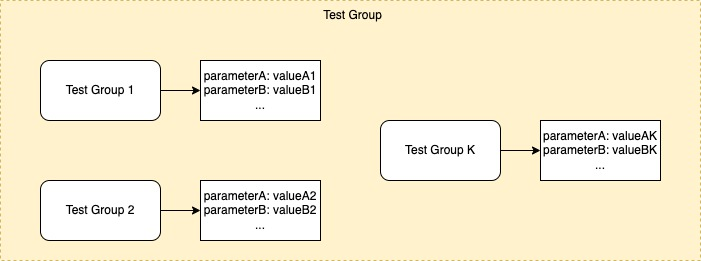
\includegraphics[height = 0.2\textwidth,width = 0.8\textwidth]{test-group}
% 	\end{figure}
% \end{frame}

\begin{frame}{Parameter}
	\begin{block}{Định nghĩa}
		\begin{itemize}
			\item Parameter đại diện cho các đặc tính của một Test Group
			\item Có thể tạo nhiều Parameter trong một Test Group
			\item Là một cặp key-value mà đối tượng có thể đọc và sử dụng
			\item Chỉ có thể sử dụng những key từ danh sách do đối tượng chuẩn bị
		\end{itemize}
	\end{block}
	\begin{block}{Ví dụ}
		color=back, color=red, enabled=true, enabled=false, etc..
	\end{block}
\end{frame}
